\documentclass[a4paper]{report}
\usepackage{setspace}
%\usepackage{subfigure}

\pagestyle{plain}
\usepackage{amssymb,graphicx,color}
\usepackage{amsfonts}
\usepackage{latexsym}
\usepackage{amsmath}
\usepackage[a4paper, margin = 3cm, bottom = 2.5cm]{geometry}
\usepackage{enumitem}
\usepackage{hyperref}
\usepackage{url}


\newtheorem{theorem}{THEOREM}
\newtheorem{lemma}[theorem]{LEMMA}
\newtheorem{corollary}[theorem]{COROLLARY}
\newtheorem{proposition}[theorem]{PROPOSITION}
\newtheorem{remark}[theorem]{REMARK}
\newtheorem{definition}[theorem]{DEFINITION}
\newtheorem{fact}[theorem]{FACT}

\newtheorem{problem}[theorem]{PROBLEM}
\newtheorem{exercise}[theorem]{EXERCISE}
\def \set#1{\{#1\} }

\newenvironment{proof}{
PROOF:
\begin{quotation}}{
$\Box$ \end{quotation}}



\newcommand{\nats}{\mbox{\( \mathbb N \)}}
\newcommand{\rat}{\mbox{\(\mathbb Q\)}}
\newcommand{\rats}{\mbox{\(\mathbb Q\)}}
\newcommand{\reals}{\mbox{\(\mathbb R\)}}
\newcommand{\ints}{\mbox{\(\mathbb Z\)}}

%%%%%%%%%%%%%%%%%%%%%%%%%%


\title{
% {\vspace{-14em} 
\includegraphics[scale=0.4]{ucl_logo.png}}\\
{{\Huge Clinical Summarisation for Intel AIPC}}\\
{\large UCL and Intel IXN Project for the NHS}\\
}
\date{Submission date: April 26th 2026}
\author{Benjamin Alexander\thanks{
{\bf Disclaimer:}
This report is submitted as part requirement for the MEng Computer Science course at UCL. It is
substantially the result of my own work except where explicitly indicated in the text.
\newline
\emph{Either:} The report may be freely copied and distributed provided the source is explicitly acknowledged
\newline  %% \\ messes it up
\emph{Or:}
The report will be distributed to the internal and external examiners, but thereafter may not be copied or distributed except with permission from the author.}
\\ \\
MEng Computer Science\\ \\
Prof. Dean Mohamedally (Internal)\\
Costas Stylianou (External)}



\begin{document}
 
\onehalfspacing
\maketitle
\begin{abstract}
GPs spent on average 25\% of their working day handling clinical paperwork and updating Electronic Patient Records (EPR) systems. This application aims to ease the stress and time taken by medical professionals by harnessing an Ambient Voice Technology (AVT) approach to record, transcribe, diarise, and summarise medical consultations to reduce time spent during and after consultations taking notes and follow-up reports. Furthermore, the appraisals feature allows doctors to generate appraisal entries by supplementing the summarisation with additional appraisal notes and tags. These entries can be viewed in the history and searched for by name or tag. Finally, by enabling the doctor to upload medical guidance documentation, the application will search for relevant guidelines to enable the GP to explore and cite medical advice based on the conversation. By engineering this project as an offline application, we expand the use case to in-home visits and ensure that all sensitive data is safe due to not requiring an internet connection for any part of the application. This application aims to reduce the time taken recording notes and inputting data into EPR systems by providing concrete transcripts, summarisations and medical advice based on the consultation.

An iterative approach allowed for flexibility in the project's development, allowing for the feedback from supervisors and healthcare professionals to be quickly integrated into the current solution. This project built on a summer project using an Intel Gaudi server running a LLM to summarise patient-doctor consultations. This was extended further to move the application onto the Windows platform, running entirely offline with the additional transcription pipeline and a RAG model for the search for relevant medical guidelines.

This project harnesses the power of Intel's AIPCs by using OpenVINO to quantise machine learning models to reduce the inference time resulting in an increase in speed and decrease in application size, producing fast and accurate summarisations of medical conversations, with medical advice provided if required.
\end{abstract}
\tableofcontents
\setcounter{page}{1}

\chapter{Introduction}
This research investigates the application of on-device machine learning to summarise clinical consultations. As a proof-of-concept, the primary objective is to evaluate the feasibility of an offline machine learning pipeline running on Intel AI PC hardware. This aims to reduce an NHS GP's workload by autonomously recording and transcribing consultations, generating clinical summaries, and retrieving medical guidance within an entirely offline environment. 

While existing cloud-based systems such as TORTUS AI, Heidi Health, and Nuance DAX Copilot highlight the utility of automated clinical documentation within healthcare, they rely on networked deployment, extensive integration, and external data processing \cite{tortus_product_2026,heidi_product_2026,dictationdirect_dax_features_2026}. In the context of the NHS, these dependencies introduce significant data governance and infrastructural challenges. Consequently, developing an offline proof-of-concept provides a mechanism to evaluate an alternative deployment architecture designed to address these specific operational constraints.

This project was developed as part of the UCL IXN in partnership with Intel with consultation from Dr. Atia Rafiq, an NHS GP and GP trainer and Dr. Tazeen Ahmed an NHS Rheumatology Care Group Lead.

\section{Problem Overview}
In a consultation, a doctor needs to listen, ask follow-up questions, reason about symptoms, and still produce a record that is accurate for later clinical use. The usual consultation flow is as follows: type and take notes during the appointment, ask follow-up questions, and reconstruct the encounter afterwards. Each of these stages has their drawbacks. Typing during the consultation interrupts eye contact and changes the rhythm of the conversation and writing notes afterwards is slow and risks losing detail.

The main idea of this project is to shift the administrative work into an on-device pipeline. The application records the conversation, transcribes and diarises (labelling sentences as doctor or patient) in real time, produces a clinical summary after the consultation, and searches uploaded guidance documents for relevant medical guidelines. In practice, the output of the consultation contains a transcript, a summary, and a link back to guidance that may help the clinician check what was discussed. This provides a practical basis for evaluating whether an offline workflow can support useful clinical documentation without relying on cloud services.

Running the full pipeline locally introduces its own problems. Large language models are expensive to run. All models must be fast to load and infer enabled by an adequately designed concurrent pipeline ensuring the application remains responsive. Retrieval and summarisation has to be fast, otherwise it becomes one more waiting step in an already busy workflow. The system also has to fit into the constraints of the target platform, a native Windows Store application built with the MSIX packaged project platform and deployed as an MSIX package on Intel AI PC hardware.

\section{Aims}
The project has three main aims:

\begin{itemize}
    \item Evaluate whether the selected models and libraries are fast enough and accurate enough to support an offline workflow in practice.
    \item Build a working proof of concept for offline clinical summarisation on Intel AIPC hardware, with a native Windows user interface and an entirely local inference pipeline.
    \item Produce a codebase and architecture that can be extended after the project, rather than a one-off demonstration that is difficult to maintain.
\end{itemize}

A personal secondary aim is established based on the project requirements. The majority of my development experience throughout my university journey is with Python and VSCode. The technical constraints of this project provide the opportunity to learn the C++ programming language, the Visual Studio environment and the MSIX Packaged Project platform. 

\section{Goals}
From those aims, I defined the following concrete project goals:

\begin{itemize}
    \item Compare candidate pre-trained medical large language models (LLMs) under different quantisation levels and select a summarisation model that is feasible on the target hardware.
    \item Build an Ambient Voice Technology (AVT) pipeline to record and transcribe conversations
    \item Build a retrieval pipeline that allows clinicians to upload medical guidance PDFs and locate relevant sections from the generated consultation summary.
    \item Provide a Windows-native interface for recording, reviewing outputs, selecting and saving external files, and browsing retrieved guidance.
    \item Structure the application so that future work, such as appraisal support or EPR integration, can be added without major rewrites.
\end{itemize}

These goals are intentionally narrower than the long-term ambitions of the product idea. For example, direct EPR integration, multilingual support, and patient-facing summaries are useful extensions, but they are not required to establish whether the core offline pipeline is viable for this proof-of-concept project.

\section{Development Methodology}
This project was set out with two phases, feasibility followed by iterative development on a 1 week cycle. Initially a feasibility study was conducted to determine whether latency and accuracy within the summarisation pipeline could remain within the requirement specification. This involved testing candidate models by measuring inference times, and evaluating performance on a summarisation benchmark.

Development began once technical this feasibility study concluded. Weekly meetings with my external supervisor and regular discussion with my internal supervisor and the NHS clients expanded the small starting feature pool. The original requirements were deliberately narrow, focusing only on local summarisation. Through demonstrations and feedback collection, the scope broadened to include AVT, medical guidance retrieval, and appraisal entries. 

The project is maintained on GitHub, which makes it practical to isolate experiments, preserve stable versions for demonstrations, and revert changes when a promising approach had flaws that required a reset to fix. This mattered most when integrating several highly linked libraries simultaneously with very different potential points of failure.

This flexible development lifecycle suited a proof-of-concept project with several unknowns and regularly evolving requirements. By prioritising high-risk ambiguities in the requirements at the start of development, a stable baseline could be set for demonstrations, thus pre-empting repository refactors due to sudden shifts in requirements.

\section{Overview}
The remainder of this report is organised as follows.

Chapter 2 reviews the background to the project, surveys comparable systems, and explains the choice of models, frameworks, and supporting libraries.

Chapter 3 defines the project requirements in detail and analyses the consequences of those requirements for the system architecture, data model, workflows, and stakeholder responsibilities.

Chapter 4 describes the design and implementation of the application, including the structure of the main components and the reasoning behind the architectural decisions.

Chapter 5 presents the testing strategy, summarises the evidence gathered during development, and identifies the main limitations of the current proof of concept.

Chapter 6 reviews the project against its original goals, critically evaluates the resulting system, and outlines the most important directions for future work.
\chapter{Context and Background Information}
% This chapter should cover background information, related work, research
% done, and tools or software selected for use in the project.
% – Provide necessary context and background information to describe
% how your project relates to what is already known or available.
% – A description of the research carried out to learn out about the nature
% of the problem(s) being investigated and potential solutions. The form
% of the research will vary widely depending on the kind of project. For
% example, it might involve searching through research publications and
% online resources, or might involve an exploration of design
% possibilities for a user interface or program structure.
% – The sources of information you are drawing on (papers, books,
% websites, etc.) should all be cited or referenced clearly. In addition,
% state how each source relates to your work and avoid the temptation
% to pad out the chapter by including sources that you didn’t make use
% of during the project.
% – If relevant, a survey of similar solutions, programs or applications to
% yours, and how yours is differentiated.
% – Introduce the software, programming languages, library code,
% frameworks and other tools that you are using. Discuss choices and
% make clear which you made use of and why.
% You should not include well known things (e.g., HTML or Java) or try to give
% tutorials on how to use a tool or code library (use references to books and
% websites for that information). Everything you include should be directly
% relevant to your work and the relationship made clear. This chapter is likely
% to be fairly substantial, perhaps 8-10 pages.

% You should provide enough background to the reader for them to understand what the project is all about. For example:
% • What problem are you solving?
% • Why are you solving it?
% • How does this relate to other work in this area?
% • What work does it build on?
% • What is the scope of your work?
% • What is included in the scope and what is outside the scope?

\section{Background Information}
\subsection{OpenVINO}
The Intel Open Visual Inference and Neural Network Optimization (OpenVINO) toolkit is an open-source software stack designed to facilitate the rapid optimisation and deployment of machine learning models on Intel AIPC hardware\cite{intel_openvino_genai_workflow_2026}. Although the original release in May 2018 focused on computer vision tasks, it has received yearly updates following industry movement towards LLMs and generative AI\cite{intel_openvino_launch_2018}. One large benefit of this toolkit is the `optimum-cli` tool, enabling the download, quantisation, and conversion to OpenVINO intermediate representation (OpenVINO IR)\cite{intel_openvino_gaudi_aipc_2024}. The tool converts any huggingface model to OpenVINO IR format. If quantisation is required, it uses the Neural Network Compression Framework to reduce the mathematical precision of the model's weights, reducing the storage size and inference time with a negligible trade-off of inference accuracy\cite{hybrid_llm_openvino_2024}. It then exports the model into a .xml file mapping the network configuration and a .bin file containing the model's weights to satisfy the OpenVINO IR format. The OpenVINO inference engine executes the OpenVINO IR model using an optimised C++ engine directly interacting with low level hardware instruction sets on Intel's AIPC system-on-a-chip (SOC) architecture\cite{intel_openvino_inference_engine_2023}.

\subsection{Intel AI PC}
The Intel AIPC series was launched in December 2023 transitioning away from the old architectures of separately dedicated CPU, GPU and RAM components and moving towards a SOC design\cite{intel_meteor_lake_2023} where the previous components and new Neural Processing Unit (NPU) all live on the same combined chip stack by the release of the Lunar Lake series in late 2024. The NPU was a new computational unit specialised for low power matrix computation, designed as a device for low power inference of small ML models\cite{intel_lunar_lake_2024}. When paired with the native OpenVINO inference engine, the Intel AIPC is a strong candidate to provide a proof-of-concept for locally hosted ML pipelines\cite{fei2024_nitro_openvino}.

\subsection{Ambient Voice Technology}
Ambient Voice Technology (AVT) is an umbrella term for the field of passive automated note taking during conversations. The standard pipeline is as follows:

\begin{figure}
    \centering
    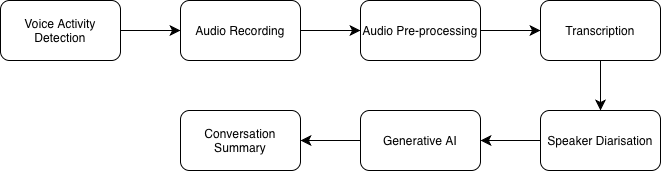
\includegraphics[width=1\linewidth]{AVT_diagram.drawio.png}
    \caption{A typical AVT workflow}
    \label{fig:AVT_diagram}
\end{figure}

This pipeline takes an audio stream as input, providing a summary as output \cite{lakhani_ai_scribes_2025}. Within the medical section this pipeline has been implemented with specialised speech-to-text and summarisation models to produce standardised medical documentation from a medical conversation \cite{tortus_product_2026}

\subsection{RAG}
Retrieval Augmented Generation (RAG) is a technique that enhances generative model outputs by first retrieving contextually relevant information from an external knowledge base and conditioning the model's generation on that retrieved context\cite{lewis_rag_2020}. This addresses a fundamental limitation of parametric LLMs. Since knowledge is fixed at training time, reliable access to domain specific or recently updated information is impossible without model retraining. The retrieval stage converts both the query and the knowledge base documents into dense vector representations (embeddings) using a semantic encoder. These embeddings capture the contextual meaning of text, enabling semantically similar passages to be located without exact keyword overlap. An approximate nearest neighbor (ANN) algorithm then searches the embedding index to surface the most contextually relevant document chunks\cite{malkov_hnsw_2020}. The retrieved chunks are passed to the LLM as additional context, enabling grounded responses anchored in verified source documents and significantly reducing the hallucination of domain-specific facts\cite{gao2023retrieval}. 

\subsection{NHS Appraisals}
Medical appraisals are an annual meetings with a supervisor aimed at retrospectively assessing challenges and lessons learnt from a personal development plan\cite{nhs_england_what_is_appraisal}. During this process, doctors must review their practice, evaluate patient and colleague feedback, and establish continuous personal development plans \cite{gmc_appraisal_guidance}. A method of reviewing their practice is through ad-hoc notes on specific consultations. An AVT solution can alleviate some of the pressure of gathering supporting information from consultations by storing reflection notes until an appraisal is required. This integration was requested by Dr. Atia Rafiq to aid her trainee GP's through this process

\subsection{Project Ambience (LLMedic)}
The prequel to this project, developed over the summer 2025 at UCL, hosted the Med42-70B model used for medical summarisation on Intel's GAUDI compute servers designed for AI acceleration on Intel hardware\cite{intel_gaudi3_2025}. This project acted as a proof-of-concept for running large AI fine-tuned medical models on Intel hardware using a web application for a client-server distribution model. The main shortfall was the hosting architecture as this server has open access to UCL students on a root level account, resulting in a solution too insecure to handle sensitive data. To remedy this, the project requires moving this model to an offline, on-device solution \cite{intel_openvino_gaudi_aipc_2024} while extending the summarisation pipeline with an AVT approach, appraisal entry system and RAG for medical advice. 

\section{Evaluation of Similar Solutions}
Evaluating the capabilities and shortfalls is essential to building a unique application that can capture the pain points of the current applications available to enable this proof of concept project to target a gap in the market. Furthermore, by analysing the current solutions, this project can position itself to develop on the successes that other applications have achieved in this growing field. 

\subsection{TORTUS AI}
TORTUS AI is an ambient medical scribe developed for the NHS as part of Great Ormond Street Hospital's (GOSH) drive for digital innovation involving a pipeline of machine learning models achieving an AVT and AI-scribe solution with complete integration into the GOSH EMIS EPR system\cite{tortus_product_2026}. This solution creates a "clinician in the loop" to systematically categorise LLM errors into risk levels targeting hallucinations and omissions from summaries during the training of their summarisation model on 13000 clinician annotated statements\cite{tortus_creola_2026}. Rollouts of this solution have shown a 23.5\% increase in face to face interaction between patients and doctors during consultations with an 8.2\% decrease in consultation length\cite{gosh_implementing_ai_2025}. In high pressure environments such as A\&E, the deployment of this solution enabled doctors to treat 13.4\% more patients per shift\cite{nia_tortus_2025}. Overall this is the leading solution for AVT and AI-scribe technologies in the NHS.

Considering the features of this project's solution, TORTUS AI does not support functionality for citing medical guidelines, or an appraisal entry solution. Furthermore, the key differentiating factor is the platform these applications will be hosted on. TORTUS uses a server-client network strategy, requiring a stable internet connection and complex network configuration within each NHS hospital and practice compared to our offline solution.

\subsection{Heidi Health}
Heidi health is a the UK's largest AVT solution founded in Australia. This solution is the UK's largest clinical rollout of AVT with the Modality Partnership, the NHS's largest GP super-partnership serving 360 GPs\cite{heidi_modality_2026}. This solution enables multi-language support along with generating subjective, objective, assessment, plan (SOAP) notes, referral letters, patient explainers and medical code suggestions with UI customisation and a large range of platforms. Due to this solution having a global scale, support for EHR integration is not yet possible\cite{deepcura_heidi_review_2026}. This platform also contains a "Context" feature allowing clinicians to upload patient documents, notes and clinical guidelines to provide the "Ask Heidi" chatbot with patient data\cite{heidi_product_2026}. Evaluating the pilot of this solution with 47 primary care doctors, Heidi state a clinicians experienced a 61\% reduction in after-hours admin and a 51\% reduction in documentation time during appointments resulting in 78\% of clinicians stating they build a better rapport with patients\cite{colcol_ai_adoption_2026}. Heidi have also recently rolled out a hybrid solution allowing Doctors to attach a proprietary clip-on microphone to capture conversations offline then connecting to the online system once convenient to then integrate with the current Heidi system\cite{wells_heidi_hardware_2026}. 

This solution trades off EPR integration for extensive UI customisation compared to TORTUS resulting in the comparison between Heidi and this project being identical to the previous comparison of TORTUS and this project. The extension that heidi provides is a workaround to gain offline capabilities, however requires the purchase and carrying of a proprietary device.

\subsection{Nuance DAX Copilot (Microsoft)}
Nuance Dragon Ambient eXperience (DAX) Copilot is an ambient AI solution by Nuance Communications, acquired by Microsoft. This harnesses the Azure's secure cloud infrastructure designed to scale with EPR integration in zero-trust security environments. In the context of our NHS domain, this solution has native integration with the EPIC EPR system through Dragon Medical One, while harnessing Microsoft's RAG capabilities within the hospital trust's database by ingesting the database based on a configuration for an enterprise-level RAG solution\cite{dictationdirect_dax_features_2026}. Total Voice Technologies, a retailer of DAX, claim that clinicians saved 7 minutes per encounter with 70\% of clinicians reporting a reduction of fatigue during and after consultations while capturing 75\% more information\cite{totalvoicetech_dax_2026}.

This is a very well rounded solution harnessing the power of Microsoft's cloud computing to create a central knowledge bank which can be automatically updated and queried. Again similar to the previous solutions, there is no native capability to handle remote consultations where a stable wifi connection and hospital network access is difficult and not guaranteed.

\subsubsection{Conclusion}
To conclude, although solutions in this field already exist, our unique approach of a completely offline open-source approach with the addition of integrating medical guidelines positions this project in a unique area. This negates the drawbacks of requiring network and server setup or proprietary devices along with the safety of sensitive data transmission over a network. After researching for completely offline on-device solutions, none were found at the time of writing for a clinical application. By attempting to capture the many benefits of these different applications while maintaining an offline solution, this project will act as a proof of concept for locally hosted AI solutions within the healthcare sector. Unfortunately due to the scope of this project, integration into current EPR system is unfeasible due to the legal challenges they create.

\section{Platforms, Models, Frameworks and Libraries}
Given the strict requirements of this project, the selection of development tools, frameworks, and libraries demanded careful evaluation. This planning phase was critical to avoid structural incompatibilities when bridging the application's many components. 

\subsection{Platform Selection}
The initial phase of development involved evaluating available platforms. Since the final product requires a native Windows application publishable to the Microsoft Store, three architectural approaches were considered:

\subsubsection{Option 1: A Fully Native Windows Packaged Application}
\begin{itemize}
    \item \textbf{Development Environment:} Visual Studio
    \item \textbf{Packaging:} MSIX packaged application
    \item \textbf{Front-End:} WinUI3 (XAML)
    \item \textbf{Back-End:} C++ with C++/WinRT / C\# with .NET
\end{itemize}
A primary advantage of a fully native approach is the streamlined deployment and testing pipeline. Unifying the front-end and back-end within a single native environment enabled easy building, packaging, deployment and debugging. Furthermore, maintaining all files within the same ecosystem facilitates rapid, iterations across the whole application stack. The main drawback of this approach is the steep learning curve. As a Python developer, transitioning to the C family of languages and developing on a new platform with a new development environment will result in slower development and debugging.

\subsubsection{Option 2: A Native Windows Front-End with a Compiled Back-End}
\begin{itemize}
    \item \textbf{Development Environment:} VS Code and Visual Studio
    \item \textbf{Packaging:} Nuitka or PyInstaller integrated into an MSIX packaged application
    \item \textbf{Front-End:} WinUI3 (XAML)
    \item \textbf{Back-End:} Python
\end{itemize}
This hybrid approach harnessed my existing proficiency in Python to handle the majority of the application development. By using my familiar VS Code environment and programming language would be optimal for my personal skill set allowing for rapid back-end prototyping and development. However, the architectural complexity of packaging a Python application into a standalone executable or library introduced severe limitations. Since the application requires managing open audio buffers and handling asynchronous data transfer between the front-end and back-end, this bridging process risked becoming cumbersome to implement and difficult to test.

\subsubsection{Option 3: A Non-Native Application Packaged for Windows}
\begin{itemize}
    \item \textbf{Development Environment:} VS Code
    \item \textbf{Packaging:} Nuitka/PyInstaller wrapped in an MSIX package to enable Microsoft Store publishing.
    \item \textbf{Front-End:} PyQt6
    \item \textbf{Back-End:} Python
\end{itemize}
A completely Python-based stack offered the most familiar development environment, but it presented substantial performance and system integration drawbacks. The front-end must handle native Windows file navigation and require seamless access to microphone permissions including features that are natively supported in a native approach but often require complex workarounds in PyQt6. Critically, the application must simultaneously manage user input, load summarisation models into the GPU, and execute a live audio transcription pipeline. Due to Python's Global Interpreter Lock, multi-threading is computationally expensive and highly restrictive, which would likely result in an unresponsive UI and unacceptable latency during live audio processing and LLM inferences.

\subsubsection{Conclusion}
To fulfil the core requirement of delivering a high-performance, Windows-native application, Option 1 was selected. Despite the steep learning curve, adopting a completely native environment (C++/C\#, WinUI3) yielded the necessary efficiency and ease of deployment. Foundational programming experience in Java and C facilitated this transition, ultimately making the development process highly effective. The performance bottlenecks of Python's GIL and the fragility of handling asynchronous audio streams across packaged Python executables were deemed too restrictive for this application's real-time requirements.

\subsection{Libraries}
To gain better understanding of the different libraries in the program, here is a brief chronological flow that the program will run. All models are downloaded and run using the OpenVINO library

\begin{itemize}
    \item \textbf{Before the application is uploaded to the Microsoft Store:}
    \begin{itemize}
        \item The models are converted to OpenVINO IR format and quantised to int4 model weights using the OpenVINO optimum-cli tool.
    \end{itemize}
    
    \item \textbf{Before a conversation begins:}
    \begin{itemize}
        \item Doctor records their voice to calculate the doctor's speech embedding (voiceprint) for future diarisation.
    \end{itemize}
    
    \item \textbf{Once a conversation begins:}
    \begin{itemize}
        \item The conversation audio is recorded using the MiniAudio library in real time.
        \item The conversation is transcribed with the Whisper-Medium model then diarised with the Speechbrain ECAPA-TDNN model in real time to generate a labelled transcript.
    \end{itemize}
    
    \item \textbf{After a conversation ends:}
    \begin{itemize}
        \item The transcript is summarised with the Med42-8b summarisation model.
        \item Any relevant guidance PDFs are uploaded and their embeddings are calculated with MedCPT.
        \item The embeddings, PDF metadata and embedding bounding boxes are stored in an SQLite database.
        \item The embeddings of the summarisation are calculated with MedCPT.
        \item The HWSNLib library enables a search the dense vector graph of embeddings to find the closest semantic matches to the summarisation within the medical guidance.
        \item The MuPDF library displays the guidance within the PDF by highlighting the areas of medical guidance that were found to be most relevant to the summarisation.
    \end{itemize}
\end{itemize}


Having established the WinUI3 and MSIX packaged application platform as the optimal architectural route, specific libraries were evaluated to support the application's specialised sub-tasks. Research was undertaken to identify the most robust and compatible tools for this native ecosystem.

\subsubsection{OpenVINO}
Because a core objective of this project is to harness the hardware capabilities of an Intel AIPC for local model inference, Intel's OpenVINO toolkit was a non-negotiable choice. This toolkit converts ML models into an Intermediate Representation (IR) specialised for Intel hardware, significantly decreasing inference latency. Since the library is only compatible with C/C++, this ruled out a C\#/.NET MSIX approach leaving a WinRT/C++ MSIX packaged application as the only viable platform choice.

Using the optimum-cli tool, models can be downloaded from HuggingFace, the industry standard repository for open-source machine learning, and quantised to specific weight sizes to greatly decrease memory usage and inference time. 

\subsubsection{MiniAudio}
To handle audio streaming and microphone input selection within the C++ backend, the miniaudio library was chosen. As an open-source, industry-standard tool, it reliably handles playback, capture, encoding, decoding, and data conversion. Its architecture as a single-header, dependency free C library allows for seamless integration. Implementation requires only a single macro definition to be instantiated within the project's scope, minimizing configuration overhead.

\subsubsection{MuPDF}
MuPDF is a lightweight and highly versatile library selected to embed a functional PDF viewer directly within the WINUI3/WinRT front-end. This is used to display relevant medical guidance documents, render bounding boxes around contextually important medical guidance sections, and support programmatic navigation between specific pages. Crucially, it achieves this while maintaining standard PDF viewer functionalities such as searching, saving, and scaling.

\subsubsection{SQLite3}
SQLite3 was implemented to store document chunk IDs, corresponding text, bounding box coordinates, PDF metadata, and the vector embeddings of user-uploaded medical guidance. By storing these embeddings alongside the raw text, SQLite3 effectively maps the semantic guidance retrieved during the vector search directly back to its source location within the raw PDF. 

Because this application operates entirely offline, traditional client-server relational databases such as PostgreSQL were unnecessary. Such databases would introduce unecessary network configuration and resource overhead. A serverless, self-contained SQL database keeps the entire retrieval pipeline strictly localised, ensuring zero-configuration access to indexed medical guidance.

\subsubsection{HNSWLib}
To power the RAG pipeline, an Approximate Nearest Neighbor (ANN) approach was required. While exact match retrieval algorithms such as kNN offer high precision, their linear scaling results in linearly slow inference times for large document sets. HNSWLib was selected as it prioritises retrieval speed without significantly sacrificing the semantic accuracy which is vital for medical contexts. It was chosen over heavier, managed vector databases to ensure the application's local footprint remained lightweight and responsive.

\subsection{Models}
\subsubsection{Med42-8B}
For the core summarization task, the Llama3 based LLM Med42-8B model pre-trained on biomedical textbooks and PubMed publications was selected. This model was chosen following a comparative analysis of the leading sub-10b parameter medical LLMs \ref{sec:med42test}. Utilising a domain-specific pre-trained LLM increases the accuracy of responses within this domain\cite{nissen2025medicine}. While the 70B model used in predecessor to this project was considered, hardware limitations of the target Intel AIPCs (32GB system RAM and 18GB VRAM) prevented loading and quantising such a large model locally. The 8B variant serves as the optimal intersection of hardware compatibility and summarisation accuracy.

\subsubsection{Whisper-Medium}
Speech-to-text transcription is handled by Whisper-Medium. This open-source model was trained on a highly diverse, multi-lingual dataset, cleanly enabling future multi-lingual support. Furthermore, OpenVINO only natively supports Whisper architectures within its \texttt{WhisperPipeline} class, this was the only viable model family. Testing across the Whisper family revealed that the "Large" variant introduced too much latency and performance overheads when running on the CPU, whereas the "Medium" model provided the ideal balance of inference speed and transcription accuracy compared to the "Base", "Normal" and "Tiny" models. Its efficiency allows the application to transcribe conversations in real time, eliminating the need to buffer and store audio files for post-processing.

\subsubsection{Speechbrain ECAPA-TDNN}
To generate labelled transcripts, a model is required to handle speaker diarisation, the process of identifying which participant is speaking at any given time. This is achieved by passing sentences of the raw audio and transcript into the ECAPA-TDNN model, which calculates the voice embeddings for each sentence. The system mathematically compares the embeddings of an unknown speaker against a pre-recorded embedding of the doctor's voice to determine whether the doctor or patient is speaking for a given sentence. This allows the application to definitively label each transcribed sentence as \texttt{[Doctor]} or \texttt{[Patient]}. Because the model is exceptionally lightweight, it runs efficiently on the CPU concurrently with the Whisper model and the rest of the application during conversation, significantly reducing post-processing delays before summarisation begins.

\subsubsection{MedCPT}
MedCPT is a domain-specific semantic information retrieval model pre-trained exclusively on biomedical data. In this pipeline, it is utilised to convert both the generated conversation summaries and the raw PDF guidelines into dense vector representations. These vectors are then mathematically searched with HNSWLib to retrieve the closest contextual match between the consultation summary and the uploaded medical guidance. By harnessing dense semantic matching rather than simple lexical matching, the system ensures that the clinical meaning behind a patient's symptoms or a doctor's recommendation is linked to the correct guidance.

\chapter{Requirements and Analysis}
This chapter elaborates on the problem introduced previously, derives a structured set of requirements from that problem, and analyses those requirements to inform the first-pass design of the application. Requirements were initially set after the introductory meeting with Costas Stylianou, then gathered iteratively through meetings with my internal supervisor (Prof.\ Dean Mohamedally), external supervisor (Costas Stylianou, Intel), and demonstrations to clinicians at NHS healthcare institutions throughout the project.

\section{Detailed Problem Statement}
Clinical documentation in UK primary care is a significant source of administrative time and burnout. GPs routinely spend a substantial portion of their working day updating Electronic Patient Records (EPR) systems, writing referral letters, and recording consultation notes. During consultations, note taking divides the clinician's attention between the patient and their method of note taking, reducing face-to-face interaction and overall consultation quality. Existing ambient voice technology (AVT) solutions such as TORTUS AI, Heidi Health, and Nuance DAX Copilot address this problem, but all depend on cloud infrastructure. This introduces three recurring barriers to adoption in NHS settings: the complexity of network and firewall configuration within each trust, the compliance of transmitting sensitive patient data over external networks, and the inability to function during home visits or in locations without a stable internet connection.

This project aims to build an open source proof of concept Windows application that records, transcribes, diarises, and summarises patient-doctor consultations entirely on-device harnessing the power of Intel AIPC hardware. The application must also allow clinicians to upload medical guidance documents and retrieve the most relevant sections based on the conversation summary using a Retrieval Augmented Generation (RAG) pipeline. By running all processing locally, the application eliminates network dependencies and simplifies data protection compliance as patient data never leaves the device.

The scope of this project is a functional proof-of-concept. It is not intended to be a production ready clinical tool, however it must be sufficiently robust and performant to demonstrate the feasibility of offline AVT in a clinical context. The application must be packaged as a native Windows Store application using the MSIX platform, built with WinUI3/C++ and have all models optimised with Intel's OpenVINO SDK.

\section{Requirements}

Requirements are organised into four categories: general requirements covering project-level constraints and deliverables, technical requirements specifying platform and hardware constraints, functional requirements describing what the application must do, and non-functional requirements specifying quality attributes the application must exhibit prioritised with the MoSCoW system. Each requirement is assigned a unique identifier for traceability.

\subsection{General Requirements}
\begin{table}[H]
\centering
\begin{tabularx}{\textwidth}{l X}
\toprule
\textbf{ID} & \textbf{Requirement} \\
\midrule
G1 & The application must be delivered as a proof-of-concept demonstrating the feasibility of offline clinical AVT on Intel AI PC hardware. \\
G2 & The application must be publishable to the Microsoft Windows Store as an MSIX packaged application. \\
G3 & Video demonstrations and presentations must be delivered to clients and supervisors on request, tailored to the target audience and iteratively refined based on feedback. \\
G4 & Workshops and presentations at relevant events must be attended to gather feedback from healthcare professionals and promote the project. \\
G5 & The application must be designed with extensibility in mind so that future developers can build upon this proof-of-concept towards an industry ready product. \\
G6 & All source code must be hosted on GitHub with a branching strategy that supports parallel feature development and rollback. \\
\bottomrule
\end{tabularx}
\caption{General requirements}
\label{tab:general-reqs}
\end{table}

\subsection{Technical Requirements}

\begin{table}[H]
\centering
\begin{tabularx}{\textwidth}{l X}
\toprule
\textbf{ID} & \textbf{Requirement} \\
\midrule
T1 & The front-end must be built with WinUI3 using XAML for the UI layer and C++/WinRT for the application logic. \\
T2 & The back-end inference pipeline must use Intel's OpenVINO toolkit to execute all machine learning models on-device. \\
T3 & The target hardware platform is an Intel AI PC with a minimum of 32\,GB system RAM, 18\,GB VRAM, and an integrated NPU. \\
T4 & All machine learning models must be converted to OpenVINO Intermediate Representation (IR) format and quantised to int4 or int8 weight precision prior to distribution. \\
T5 & The application must operate entirely offline with zero network communication to external services during all use cases. \\
T6 & The development environment must be Microsoft Visual Studio with the MSIX packaging toolchain. \\
T7 & A pre-trained medical LLMs with no more than 10 billion parameters must be evaluated and selected to fit within the memory constraints of T3. \\
T8 & The speech-to-text model must be from the Whisper family due to OpenVINO's native \texttt{WhisperPipeline} support. \\
T9 & The application must record a conversation and process the audio stream in real time, providing building the transcription live during the conversation. \\
T10 & The concurrent architecture must allow all models to run simultaneously in memory to avoid loading overheads. \\
T11 & The doctor's voice embedding must be encrypted.
\bottomrule
\end{tabularx}
\caption{Technical requirements}
\label{tab:technical-reqs}
\end{table}

\subsection{Functional Requirements}

Functional requirements are prioritised using the MoSCoW method. \textit{Must Have} requirements define the minimum viable product. \textit{Should Have} requirements add significant value but are not blocking. \textit{Could Have} requirements are desirable extensions that fall outside the core scope.

\subsubsection{Must Have}

\begin{table}[H]
\centering
\begin{tabularx}{\textwidth}{l X}
\toprule
\textbf{ID} & \textbf{Requirement} \\
\midrule
F1 & The user must be able to select an audio input device from any microphone connected to the laptop, including the built-in microphone as default. \\
F2 & The application must diarise the conversation by labelling each transcribed segment as either \texttt{[Doctor]} or \texttt{[Patient]}, based on a pre-recorded voice embedding of the doctor. \\
F3 & The user must be able to record their voice before a consultation to generate the voice embedding used for diarisation. \\
F4 & The recorded voice embedding must be saved and encrypted locally for use in future conversation. \\
F5 & On completion of a conversation, the application must generate a clinical summary of the diarised transcript using a pre-trained medical LLM. \\
F6 & The user must be able to save the transcript and summary to a user-specified location on the local file system. \\
F7 & A default save location must be available for the user to select. \\
F8 & The relevant NICE Guidelines must be highlighted based on the summary. \\
F9 & The user must be able to remove previously uploaded medical guidance documents. \\
F10 & After summarisation, the application must retrieve and display the sections of uploaded medical guidance most relevant to the consultation summary, using a semantic search pipeline. \\
F11 & Retrieved guidance must be displayed within an embedded PDF viewer with the relevant sections visually highlighted. \\
F12 & The application must provide clear visual feedback during long-running operations (transcription, summarisation, guidance retrieval) so the user is aware of the current processing state. \\
F13 & The application must provide a responsive, intuitive Windows-native user interface suitable for clinicians with varying levels of technical proficiency. \\
F14 & A help section with a guidance on how to use the application, and an information section with the relevant legal disclaimers and model information must be accessible through the application. \\
\bottomrule
\end{tabularx}
\caption{Functional requirements (Must Have)}
\label{tab:func-must}
\end{table}

\subsubsection{Should Have}

\begin{table}[H]
\centering
\begin{tabularx}{\textwidth}{l X}
\toprule
\textbf{ID} & \textbf{Requirement} \\
\midrule
F15 & The user should be able to create appraisal entries from a completed summarisation, attaching free-text notes and tags to each entry. \\
F16 & Appraisal entries should be searchable by name and filterable by tag. \\
F17 & The user should be able to view, edit, and delete individual appraisal entries, and delete all entries at once. \\
F18 & The application should support the upload and semantic searching of non-NICE medical guidance PDFs alongside NICE guidelines. \\
\bottomrule
\end{tabularx}
\caption{Functional requirements (Should Have)}
\label{tab:func-should}
\end{table}

\subsubsection{Could Have}

\begin{table}[H]
\centering
\begin{tabularx}{\textwidth}{l X}
\toprule
\textbf{ID} & \textbf{Requirement} \\
\midrule
F19 & Multi-lingual transcription and translation support during conversation. \\
F20 & Voice recording of post-consultation notes appended to the transcript. \\
F21 & A patient-facing plain-language summary generated alongside the clinical summary. \\
F22 & A voice-activated trigger (e.g.\ ``Hey Ambience'') to begin recording without pressing a button. \\
F23 & Integration with EPR systems to export summaries directly into patient records. \\
\bottomrule
\end{tabularx}
\caption{Functional requirements (Could Have)}
\label{tab:func-could}
\end{table}

\subsection{Non-Functional Requirements}

\begin{table}[H]
\centering
\begin{tabularx}{\textwidth}{l l X}
\toprule
\textbf{ID} & \textbf{Category} & \textbf{Requirement} \\
\midrule
NF2 & Performance & Summary generation must complete within 90 seconds of the conversation ending for a consultation of up to 15 minutes. \\
NF3 & Performance & Semantic search over uploaded guidance documents must return results within 3 seconds. \\
NF4 & Performance & The UI must remain responsive (no freezing or dropped frames) during all background processing operations including recording, transcription, and summarisation. \\
NF5 & Performance & The application must start and load all ML models into memory within 60 seconds of launch. \\
NF6 & Security & All persisted data (transcripts, summaries, appraisal entries, voice embeddings) must be encrypted at rest on the local file system. \\
NF7 & Security & The application must make zero outbound network requests during operation, ensuring patient data never leaves the device. \\
NF8 & Security & Deletion of appraisal entries and associated data must be permanent and non-recoverable. \\
NF9 & Usability & The interface must be navigable by clinicians with no prior training, using standard Windows UI conventions and clear labelling. \\
NF10 & Usability & All primary workflows (start recording, stop recording, view summary, view guidance) must be achievable within three clicks from the main screen. \\
NF11 & Reliability & The application must handle errors during model inference (e.g.\ out-of-memory) gracefully, displaying an informative error message without crashing. \\
NF12 & Maintainability & The codebase must follow a modular architecture with separation between UI, audio processing, model inference, and data persistence layers to support future extension. \\
NF13 & Portability & The application must run on any Intel AIPC meeting the hardware specification in T3 without requiring manual driver or dependency installation by the end user. \\
\bottomrule
\end{tabularx}
\caption{Non-functional requirements}
\label{tab:nfr}
\end{table}

\section{Requirement Analysis}

The defined requirements were analysed to identify the key data entities, user workflows, and architectural constraints that would inform the design of the application. This section documents that analysis and the reasoning behind the early design decisions it produced.

\subsection{Data Entities}
Working through the functional requirements, 7 core data entities that the application needs to manage:

\begin{table}[H]
\centering
\begin{tabularx}{\textwidth}{l X}
\toprule
\textbf{Data Entity} & \textbf{Description \& Requirements} \\
\midrule
Audio buffers & Raw audio captured from the microphone in real time into an audio buffer, consumed by the transcription pipeline and discarded after processing. No long-term storage is needed since the transcript serves as the persistent record (F2). \\
Transcripts & Speaker-labelled text segments are produced during recording. These grow incrementally as the conversation progresses and are finalised when recording stops (F2, F3, F6). \\
Summaries & Clinical summaries generated from the finalised transcript by the Med42-8B model. Each summary is associated with exactly one transcript (F5, F6). \\
Voice embeddings & A fixed-length vector representing the doctor's voice, computed once during enrolment and reused across all subsequent conversations for diarisation. This must be encrypted on device (F3, F4, NF6). \\
Guidance documents & User-uploaded PDF files. Each document is chunked into text segments, and each segment has a corresponding dense vector embedding and bounding box coordinates mapping it back to a location in the source PDF (F7, F8, F9, F10). \\
Appraisal entries & Structured records containing a name, summary text, free-text notes, one or more tags, and a creation timestamp stored in a JSON format. These must support search and filtering (F15, F16, F17). \\
User preferences & Configuration state including the selected microphone device and default save location. (F1, F6) \\
\bottomrule
\end{tabularx}
\caption{Data entities and storage requirements}
\label{tab:data-entities}
\end{table}

This breakdown led to a split storage strategy. Guidance document metadata, text chunks, embeddings and bounding boxes are well-suited to a relational schema and are stored in an SQLite database. Large binary objects (PDF files, model weights) remain on the file system within the sandbox of the MSIX packaged project platform. Audio buffers, transcripts and summarisations are transient and held only in memory unless saved by the user to their specified save location.

\subsection{User Workflow Analysis}
I traced the primary user workflows through the functional requirements to determine how many distinct views the application needs and what each view must support.

\subsubsection{Conducting a consultation (F1--F6, F12)}
The clinician selects a microphone, starts recording, and conducts the consultation. When the consultation ends, the clinician stops recording and the summary is generated. The clinician reviews both the transcript and summary and optionally saves them. This workflow requires a single primary view with recording controls, a "recording in progress" pane, a summary pane, and status indicators.

\subsubsection{Retrieving medical guidance (F7-F10)}
After summarisation, the clinician navigates to a guidance view from the summarisation view where the most relevant sections of their uploaded medical guidance are listed by relevance. Selecting a result opens the corresponding PDF with the matched section highlighted. This requires a split-panel view: a ranked result list on the left and an embedded PDF viewer on the right.

\subsubsection{Managing appraisals (F15--F17)}
The clinician creates an appraisal entry from a the summarisation view, adding notes and tags. They can later return to browse, search, edit, or delete entries from any view in the application. This requires a dedicated view with a searchable and filterable grid of appraisal cards and dialog-based CRUD operations.

\subsubsection{Modifying persistent settings (F1, F3, F7, F14)}
The clinician wishes to change the default save location, microphone input or re-record the voice embedding. This can be achieved with a flyout settings menu, with the settings icon persisting in the top corner throughout the application. 

\subsection{Threading and Real-Time Constraints}
Requirements F2 and NF1 demand that audio is captured and transcribed with no more than 5 seconds of latency, while NF4 requires the UI to remain responsive throughout. On a single thread this is impossible as model inference would block the UI thread. Furthermore, the Med42-8B summarisation model must be permenantly loaded onto the GPU as load times are upwards of 15 seconds. I therefore propose the following concurrency architecture

\begin{itemize}
    \item A \textbf{UI thread} managed by the WinRT framework, handling all rendering and user interaction.
    \item An \textbf{audio capture thread} that continuously reads from the microphone and fills a shared buffer throughout the conversation.
    \item A \textbf{transcription thread} that consumes buffered audio, runs inference via Whisper-Medium then diarisation via ECAPA-TDNN, and dispatches labelled text back into a buffer in UI thread.
    \item A \textbf{summarisation thread} that loads the Med42-8B summarisation model into the GPU from program launch, then runs Med42-8B inference after the conversation ends, dispatching the result to the UI thread on completion.
    \item A \textbf{RAG thread} that computes the summary embedding, queries the HNSWLib index, and retrieves matched guidance chunks.
\end{itemize}

The first 4 threads must run concurrently during a conversation. The RAG thread then runs sequentially after the conversation ends but must still execute off the UI thread to maintain responsiveness. Communication between threads and the UI thread uses the WinUI3 dispatcher to safely update UI elements from background threads.

This threading model also maps naturally onto the heterogeneous compute resources of the Intel AI PC: the transcription model runs on the CPU, summarisation runs on the GPU, and the diarisation model and embeddings model runs on NPU.

\subsection{Offline Constraint Implications}
The offline requirement (T5, NF7) has cascading implications across the architecture:

\begin{itemize}
    \item All four ML models (Whisper-Medium, ECAPA-TDNN, Med42-8B, MedCPT) and their weights must be bundled with the application at install time and loaded from local storage.
    \item No client-server database is needed. SQLite runs in-process with zero configuration, which satisfies both the offline constraint and the portability requirement (NF13).
    \item The RAG index must be built and queried locally. HNSWLib provides in-memory approximate nearest neighbour search without requiring a server process, based on the MedCPT embeddings generated.
    \item There is no telemetry, crash reporting, or update mechanism that contacts an external server. Updates are distributed through the Microsoft Store's standard MSIX update channel.
\end{itemize}

\subsection{Security Considerations}
Requirements NF6-NF8 establish the data protection baseline. Since all data remains on-device, the primary threat model concerns unauthorised local access to the machine (e.g.\ a lost or stolen laptop). The following precautions must be taken to ensure external access to data within the application is safe.

\begin{itemize}
    \item Transcripts, summaries, and appraisal entries stored in the SQLite database must be encrypted. The MSIX application sandbox provides some isolation, but explicit encryption adds a defence in depth layer.
    \item The voice embedding file must also be encrypted, as it constitutes biometric data.
    \item The ``Delete All Appraisals'' operation (F17) must overwrite data rather than simply marking records as deleted, to prevent forensic recovery (NF8).
\end{itemize}

\section{Requirements Traceability Matrix}

Table~\ref{tab:rtm} maps each requirement to the design decisions and system components that address it. This provides forward traceability from requirements to design, ensuring every requirement has a corresponding implementation strategy and no design decision exists without a motivating requirement.

\begin{longtable}{l p{5.2cm} p{6.8cm}}
\toprule
\textbf{Req.} & \textbf{Design Decision} & \textbf{Realising Component(s)} \\
\midrule
\endfirsthead
\toprule
\textbf{Req.} & \textbf{Design Decision} & \textbf{Realising Component(s)} \\
\midrule
\endhead
\midrule
\multicolumn{3}{r}{\textit{Continued on next page}} \\
\bottomrule
\endfoot
\bottomrule
\caption{Requirements traceability matrix mapping requirements to design decisions and components.}
\label{tab:rtm}
\endlastfoot
G1 & Proof-of-concept scope; offline-first architecture & Full application pipeline \\
G2 & MSIX packaging with WinUI3 & Visual Studio MSIX project template \\
G5 & Modular architecture with separated concerns & Layered component structure (UI, inference, data) \\
G6 & Git branching strategy & GitHub repository with feature branches \\
\midrule
T1 & Native Windows front-end & WinUI3 XAML views, C++/WinRT code click and state handlers \\
T2 & On-device inference engine & OpenVINO C++ API \\
T3 & Hardware based model selection & Int4/int8 quantised models sized for 32\,GB RAM, 18\,GB VRAM target device \\
T4 & Pre-distribution quantisation pipeline & OpenVINO \texttt{optimum-cli} conversion \\
T5 & No network calls; all models bundled locally & Bundled model weights in MSIX package; SQLite in-process database; HNSWLib in-memory index \\
T7 & Sub-10B parameter constraint & Med42-8B selected after benchmarking \\
T8 & Whisper family constraint & Whisper-Medium via OpenVINO \texttt{WhisperPipeline} \\
\midrule
F1 & Device enumeration at startup & MiniAudio.h device listing API \\
F2 & Streaming audio capture with real-time transcription & Audio capture thread $\rightarrow$ shared buffer $\rightarrow$ transcription thread running Whisper-Medium and ECAPA-TDNN \\
F3 & Cosine similarity of voice embeddings & ECAPA-TDNN model comparing per-segment embeddings against enrolled doctor embedding \\
F4 & Voice enrolment workflow & Dedicated UI dialog, ECAPA-TDNN embedding computation, encrypted local storage of embedding \\
F5 & Post-conversation LLM inference & Summarisation thread running Med42-8B on GPU via OpenVINO \\
F6 & File save dialog & Windows native file picker via WinRT API \\
F7, F8 & Document management UI & Guidance view with upload/delete controls, SQLite metadata table, file-system PDF storage \\
F10 & Semantic search pipeline & MedCPT embedding of summary $\rightarrow$ HNSWLib ANN query against guidance embeddings \\
F11 & Embedded PDF viewer with highlighting & MuPDF rendering with bounding-box overlays \\
F12 & Async processing with UI feedback & Progress indicators and status text updated from background threads via WinUI3 dispatcher \\
F13 & Three-view navigation structure & NavigationView with Recording, Appraisals, and Guidance pages \\
F15-F17 & Appraisal CRUD with tagging & JSON appraisals storage, tag filtering and sorting, dialog-based CRUD modifications \\
F18 & Generic PDF support in RAG & MedCPT chunking and embedding pipeline applied to any uploaded PDF, not only NICE documents \\
\midrule
NF1 & Streaming transcription with $\leq$5\,s latency & Dedicated transcription thread; Whisper-Medium int8 on CPU; buffered audio segments \\
NF2 & Summary within 90\,s & Med42-8B int4 on GPU; prompt engineering to constrain output length \\
NF3 & Guidance retrieval within 3\,s & Pre-indexed HNSWLib graph; MedCPT embedding computation \\
NF4 & UI never blocks & Multi-threaded architecture, all inference initiated off the UI thread, dispatcher-based UI updates \\
NF5 & Startup model loading within 60\,s & Early model loading on application launch in background threads \\
NF6 & Encryption at rest & Encrypted voice embedding file \\
NF7 & Zero outbound network traffic & No HTTP/socket calls in codebase, MSIX sandbox network isolation \\
NF8 & Secure deletion & Data overwrite on delete operations rather than soft-delete \\
NF9, NF10 & Intuitive three-click workflows & Standard WinUI3 controls, NavigationView, minimal dialog depth \\
NF11 & Graceful error handling & Try-catch around OpenVINO inference calls, user-facing error dialogs \\
NF12 & Modular codebase & Separated UI layer, audio module, inference module, data-access module \\
NF13 & No manual dependency install & All dependencies bundled in MSIX package \\
\end{longtable}

\section{Use Cases}

The application targets any clinical consultation where a doctor and patient interact verbally and a written record is required afterward. The following use cases illustrate the two primary deployment contexts.

\subsection{Use Case 1: A GP Consultation}
A GP opens the application on their Intel AIPC at the start of a clinical session. The application loads the ML models during startup. Before the first patient enters, the GP records a short voice sample to register their voice embedding for diarisation. When the patient arrives, the GP clicks \textit{New Recording} and selects the laptop's built-in microphone. When the consultation ends, the GP clicks \textit{Finish Recording}. The application generates a clinical summary, and the GP reviews it alongside the transcript. The GP then navigates to the Guidance view, where the application highlights the most relevant NICE guideline sections based on the summary. The GP saves the transcript and summary to a local folder for later entry into the EPR system. If applicable, the GP creates an appraisal entry with notes and tags for their professional development portfolio.

\subsection{Use Case 2: A Home Visit Consultation}
A GP conducts a home visit where no internet connection is available. Because the application runs entirely offline, the full pipeline functions identically to a surgery consultation. The GP uses the laptop microphone to record the conversation. After the visit, the GP reviews the summary and guidance results. On returning to the surgery, the GP saves the outputs and transfers them to the EPR system. This use case demonstrates the core differentiator of this application over existing cloud-dependent solutions.
\include

\bibliographystyle{unsrturl}
\bibliography{main.bib}

\end{document}